\documentclass{standalone}

\usepackage{tikz,tikzpeople}
\usetikzlibrary{arrows.meta,matrix,backgrounds,fit,shapes,positioning}


\begin{document}
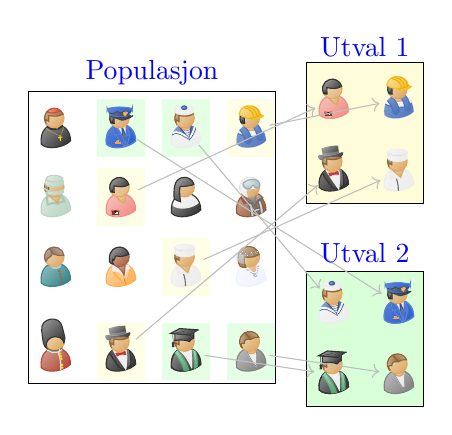
\begin{tikzpicture}
   \tikzstyle{sel}=[draw]
   \tikzstyle{pn}=[outer sep=3mm]
   \tikzstyle{ar}=[gray!50,->]
   \tikzstyle{sel}=[rectangle,fill=yellow!10]
   \tikzstyle{sel2}=[rectangle,fill=green!10]
   \tikzstyle{head}=[text=blue]
   \tikzstyle{sample}=[draw,node distance=3mm]

   \matrix (pop) [draw,matrix of nodes,row sep=3mm,column sep=4mm] {
      \node [pn,priest] {} ; &
      \node (p2t) [pn,conductor] {} ; &
      \node (p1t) [pn,sailor] {} ; &
      \node (p2) [pn,builder] {} ; \\
      \node [pn,surgeon] {} ; &
      \node (p1) [pn,nurse] {} ; &
      \node [pn,nun] {} ; &
      \node [pn,pilot] {} ; \\
      \node [pn,charlie] {} ; &
      \node [pn,alice] {} ; &
      \node (p4) [pn,chef] {} ; &
      \node [pn,bride] {} ; \\
      \node [pn,guard] {} ; &
      \node (p3) [pn,groom] {} ; &
      \node (p3t) [pn,graduate] {} ; &
      \node (p4t) [pn,bob] {} ; \\
   } ;
   \node (ref) [right=of pop] {};
   \matrix (sam) [sample,above=of ref,matrix of nodes,row sep=3mm,column sep=4mm,fill=yellow!15] {
      \node (s1) [pn,nurse] {} ; &
      \node (s2) [pn,builder] {} ; \\
      \node (s3) [pn,groom] {} ; &
      \node (s4) [pn,chef] {} ; \\
   } ;
   \matrix (sam2) [sample,below=of ref,matrix of nodes,row sep=3mm,column sep=4mm,fill=green!15] {
      \node (t1) [pn,sailor] {} ; &
      \node (t2) [pn,conductor] {} ; \\
      \node (t3) [pn,graduate] {} ; &
      \node (t4) [pn,bob] {} ; \\
   } ;
   \begin{scope}[on background layer]
      \node  [fit=(p1) (p1), sel]{};
      \node  [fit=(p2) (p2), sel]{};
      \node  [fit=(p3) (p3), sel]{};
      \node  [fit=(p4) (p4), sel]{};
      \node  [fit=(p1t) (p1t), sel2]{};
      \node  [fit=(p2t) (p2t), sel2]{};
      \node  [fit=(p3t) (p3t), sel2]{};
      \node  [fit=(p4t) (p4t), sel2]{};
   \end{scope}
   \draw [ar] (p1) -> (s1) ;
   \draw [ar] (p2) -> (s2) ;
   \draw [ar] (p3) -> (s3) ;
   \draw [ar] (p4) -> (s4) ;
   \draw [ar] (p1t) -> (t1) ;
   \draw [ar] (p2t) -> (t2) ;
   \draw [ar] (p3t) -> (t3) ;
   \draw [ar] (p4t) -> (t4) ;
   \node [above of=pop,head,node distance=21mm] {Populasjon} ;
   \node [above of=sam,head,node distance=11mm] {Utval 1} ;
   \node [above of=sam2,head,node distance=11mm] {Utval 2} ;
\end{tikzpicture}
\end{document}
